\documentclass[titlepage,a4paper]{article}
\usepackage[nottoc,numbib]{tocbibind}
\usepackage{graphicx}
\usepackage{float}
\usepackage{listings}
\usepackage[utf8]{inputenc}
\usepackage{hyperref} % Required for adding links and customizing them

 
\author{
\textbf{Group 31} \\
Hugo Sandelius, hugosa@kth.se \\ 
Simon Forssell, sifo@kth.se \\
}

\begin{document}


\begin{titlepage}
\begin{center}

\includegraphics[width=2.5cm]{KTH_Logotyp_Sv_2013.eps}\\[1.5cm]
\textbf{\LARGE Comparison of algorithms for automated university scheduling}\\
\vfill
{\Large Hugo Sandelius}\\
{\Large Simon Forssell}\\[3cm]
{\large Degree Project in Computer Science, DD143X}\\[0.07cm]
{\large Supervisor: Pawel Herman}\\
{\large Examiner: Örjan Ekeberg}\\[3cm]
{\large CSC, KTH \today}
\end{center}
\end{titlepage}

%\maketitle

\begin{abstract}
Timetable generation is a common real-world problem, that has been shown to be hard to solve. In a scheduling algorithm, various constraints related to scheduling are the inputs and a schedule satisfying these constraints is the output.
In this report, two algorithms for timetable generation are compared: Tabu Search and a Genetic Algorithm. How well the algorithms perform for generating schedules from constraint input of different sizes is assessed, as well as how the performance of the algorithms is affected by varying parameters of the algorithm.
The major conclusion drawn is that there is no major difference between how well Tabu Search and the Genetic Algorithm scale when faced with a larger input size.
\end{abstract}

\tableofcontents{}

\pagebreak
\section{Introduction}
Timetables are used in many different areas, for example:

\begin{itemize}

  \item Public transport timetables - a list of times and routes connecting places. Travelers can use this to plan how to go from point A to point B.
  \item Broadcast scheduling - used by television and radio stations to schedule when shows and commercials are broadcasted. Often certain shows are to be broadcasted at the same time every day or week.
  \item University timetables - listing all the classes together with time and location so that students know when and where to be. 

\end{itemize}
To put together a good schedule is a complex problem and it is very hard to do by hand. A multitude of factors need to be taken into account, e.g. not having one person do two different tasks at the same time, or to spread out different tasks across a schedule. It is not surprising that we let computers do this for us. In fact the problem is so complex there probably does not even exist an algorithm that will create an optimal timetable in a reasonable amount of time. This is because this scheduling problem belongs to a class of problems called \emph{NP-hard}\cite{guidedSearch09}  and a consequence of this is that as the problem size grows, the time it takes to find an optimal solution increases exponentially. \\\\
This means that it will not be possible to find an optimal solution, instead an approximate solution must be searched for. But it is not immediately clear what an optimal solution is. What an optimal solution means certainly differs depending on what the timetable is going to be used for. This report will look into what makes a good university timetable and also go over a few methods of how to generate one. \\\\
The report will compare how well two different scheduling algorithms perform for scheduling problems of different sizes. The time taken to generate schedules of various sizes will be assessed, as well as how the solution changes over the running time of the algorithm. This gives an idea of how long time it takes to generate solutions of varying quality. \\\\
First the report will measure how well the algorithm performs on a small problem size, and then see how well it scales up when applied to a significantly larger problem size.
The problems will be artificially generated by us, with inspiration from how the input files to the KTH scheduling department looks, and will be defined in more detail in the Method section. \\\\
The following algorithms will be compared, each of which address the problem from a separate angle.\\\\
\emph{Tabu Search} is a variant of a local search algorithm, which does a local search around at a solution’s neighbours to try and find better solutions. It complements this with marking certain areas as “tabu”, which means it should not be visited again\cite{aTabuSearch07}. Tabu search is used by the open source scheduling software Drools Solver (now OptaPlanner)\cite{website:timetabling-software-survey}. \\\\
\emph{Genetic algorithms} mimics the biological process of natural selection. The commercial scheduling software \emph{gp-Units} utilizes a genetic algorithm\cite{website:timetabling-software-survey}.\\\\
Tabu Search and Genetic Algorithms are both algorithms that are commonly used for optimization problems. Since this is a core part of the scheduling problem, they are commonly used for this task. There is also a lot of existing literature about using them for timetable generation. They have two quite different approaches to solving the problem, and thus would be interesting to compare.
These algorithms will be described in detail in the Background section.

\pagebreak
\section{Background}
Automated scheduling is a very well researched subject, especially in the university setting. There are numerous reports written on the various aspects of this topic, most of them in the form of detailed descriptions of algorithms solving the scheduling problem\cite{guidedSearch09}\cite{anApp05}.\\\\
Although scheduling problems have been studied since the 1960s\cite{efficient03}, the first computer-enabled scheduling systems were established in the late 1980s\cite{timeTableInfo06}. For traffic planning, there are a number of widely-used systems. Currently used systems are for example \emph{HAFAS}, used in the European railway sector, and \emph{EFA}, used for local traffic planning in many European cities. These use graph-based approaches, using versions of Dijkstra’s Algorithm combined with heuristics to try and find a good approximation of the shortest path between two physical positions\cite{timeTableInfo06}. \\\\
However, for university scheduling, most universities have developed their own solution\cite{efficient10}. The scale of the problem, as well as the constraints involved, vary widely and so does the solution approaches. However, the core of any scheduling algorithm is a combinatorial problem that must be solved by some algorithm. Some of the different algorithms that can be commonly found in scheduling litterature are \emph{local search techniques}, \emph{Tabu search}, \emph{genetic algorithms}, \emph{constraint programming} and \emph{goal programming}\cite{efficient03}. \\\\
Genetic Algorithms and Tabu Search represent two quite different approaches to the problem, although they both utilize an evaluation function to evaluate the solution in each step, and have a current best solution which is improved as the algorithm iterates.

\subsection{Genetic Algorithms}
Genetic algorithms were first used by J. H. Holland in 1975\cite{timetabling02}.\\\\
The algorithm work on a set of potential solutions. This set is called a population and each solution is represented by a chromosome. Every separate property of a specific solution is stored in the string of genes making up the chromosome. The algorithm starts off with an, often randomly generated, initial solution. A function then calculates the fitness of each chromosome by evaluating the chromosome’s solution. Chromosomes with high fitness have a higher chance of being selected for “breeding” and thereby passing on their genes to the next generation of the population. When creating the new population several genetic operators could be used, for example crossover or mutation\cite{solving12}.  \\\\
\textbf{Crossover} generates new chromosomes by swapping genes between two or more parent chromosomes. There are different ways to select which genes to swap. Picking some point in the gene string and swapping all genes beyond that point or swapping all genes within some interval are two common methods. It is also possible to randomly swap genes so that the probability of a swap is set by a mixing rate. \\\\
\textbf{Mutation} works by changing the values of the genes to something other than their initial values. Whether a gene should be changed or not is determined by probability\cite{anApp05}. \\\\
The process then starts over again with calculating the fitness of each chromosome. The average quality of the solutions will increase with every new generation. The population continues to evolve like this until an optimal solution is found, the number of iterations reaches a set limit, or some other stopping condition is met. \\\\
\subsection{Tabu Search}
Tabu Search is a search algorithm that was originally formalized by Fred W. Glover in 1989\cite{tabuSearch89}. \\\\
Tabu Search is a local search algorithm. Local searches takes a possible solution to a problem and evaluate its’ neighbors, by assigning an evaluation score to each of them, in order to see if they are a better solution. Neighbors in this case means solutions with some minor difference from the solution in question. If a neighbor has a higher evaluation score, and thus is a better solution, it becomes the new current solution, and in the next iteration neighbors to this solution are evaluated. This continues until some stopping criteria is fulfilled, similar to genetic algorithms. \\\\
Picking which neighbors should be evaluated in each iteration is a key part of local search algorithms, and this is where Tabu Search comes in.
In Tabu Search, we keep track of previously visited solutions in a tabu list. Any solution in the tabu list will not be visited again until a certain condition has been fulfilled, for example a certain number of solutions having been visited. This keeps the local search from getting stuck in a local optimum or a plateau, and helps it expand the search to other regions\cite{geneticVS99}. 

\pagebreak
\section{Method}
A program is developed that takes user input, consisting of course information and constraints, and generates schedules using two different algorithms as they are described in the Background section. The input consists of a list of classrooms and their capacities, a list of programs and their courses, and the lessons in each course, with each lesson being assigned a teacher and a number of students in the lesson. The total amount of weeks the schedule should be planned for is also included.
The schedules assigns lessons to four possible slots each day. \\\\
\subsection{Constraints}
The hard constraints, i. e. the ones which has to be fulfilled by the algorithm to be considered as a possible solution, are:
\begin{itemize}
  \item All lessons must be assigned a time
  \item A classroom must hold at least as many students as are planned for the lesson
  \item Only one lesson in one program at the same time
  \item A teacher may only teach one class at a time
\end{itemize} 
\medskip
The soft constraints, which are used to evaluate the schedule but are not absolutely necessary to fulfill, are:
\begin{itemize}
  \item The amount of free periods, i.e. unscheduled time between classes in a day for students, should be minimized
  \item There should preferably not be more than one lesson in the same course in a day
\end{itemize}
\medskip
After the schedule is generated, the program assesses how well the various soft constraints were fulfilled. If a perfect schedule, i. e. one where all soft and hard constraints are fulfilled, can be generated in a reasonable time, the amount of time and iterations of each algorithm is compared. \\\\
\subsection{Constraint files}
Two different input files of increasing sizes is used to generate the schedules. The input files are artificial, but constructed with inspiration from how the input to the KTH scheduling system works.
A script which randomly generates constraints is used to generate the constraints. The script randomly generates a schedule according to the following input:
\begin{itemize}
  \item \texttt{programs} decides the amount of programs.
  \item \texttt{courses-low} and \texttt{courses-high} decide the upper and lower bounds of the amount of courses in each program. The actual value is randomized between the two.
  \item \texttt{lessons-low} and \texttt{lessons-high} decide the upper and lower bounds on the amount of lessons.
  \item \texttt{big-prob}, the probability that a class will be \emph{big}
  \item \texttt{small-cap-low} and \texttt{small-cap-high} decide the upper and lower bounds on the required capacity of a \emph{small} class.
  \item \texttt{big-cap-low} and \texttt{big-cap-high} decide the upper and lower bounds on the required capacity of a \emph{big} class.
  \item Each course has two different teachers. \texttt{second-teacher-low} and \texttt{second-teacher-high} is the upper and lower bounds on the probability that each lesson in a given course will be given by the \texttt{second teacher}.
  \item \texttt{weeks} decide the time period, in amount of weeks, that the schedule should cover.
\end{itemize} 
The small input file was generated with the following input: \\\\
\medskip
\begin{tabular}{| l | c |}
  \hline
  programs & 3 \\
  \hline
  courses-low & 2 \\
  \hline
  courses-high & 4 \\
  \hline
  lessons-low & 7 \\
  \hline  
  lessons-high & 15 \\
  \hline  
  big-prob & 0.72 \\
  \hline  
  small-cap-low & 50 \\
  \hline  
  small-cap-high & 100 \\
  \hline  
  big-cap-low & 150 \\
  \hline  
  big-cap-high & 200 \\
  \hline  
  second-teacher-low & 0.6 \\
  \hline  
  second-teacher-high & 1.0 \\
  \hline
  weeks & 4 \\
  \hline
\end{tabular}
\medskip \\
The large input file was generated with the following input: \\\\
\medskip
\begin{tabular}{| l | c |}
  \hline
  programs & 6 \\
  \hline
  courses-low & 3 \\
  \hline
  courses-high & 5 \\
  \hline
  lessons-low & 15 \\
  \hline  
  lessons-high & 20 \\
  \hline  
  big-prob & 0.72 \\
  \hline  
  small-cap-low & 50 \\
  \hline  
  small-cap-high & 100 \\
  \hline  
  big-cap-low & 150 \\
  \hline  
  big-cap-high & 200 \\
  \hline  
  second-teacher-low & 0.6 \\
  \hline  
  second-teacher-high & 1.0 \\
  \hline
  weeks & 10 \\
  \hline
\end{tabular}
\medskip \\

The constraints are represented by a JSON-file with the following structure:

\begin{verbatim}
{
  "programs" : [
      {
      "program" : "CDATE1",
      "courses" : [
        {
          "name" : "inda",
          "lessons" : [
            {
              "teacher" : "Gustav Gustavsson",
              "capacity" : 200
            }      
          ]
        }
      ]
    }
  ],
  "classrooms" : [
    {
      "name" : "D1",
      "capacity" : 200
    }
  ],
  "weeks" : 1
}

\end{verbatim}
Since both algorithms has elements of randomness they are run 10 times with each input file, after which the average result is calculated, to avoid the impact of chance on the algorithms. \\\\

\subsection{Implementation}
The program is implemented in the Java programming language, using the Tabu Search library OpenTS and the Genetic Algorithms library JGap. The source code is available at \href{https://github.com/hugoflug/schedule}{github.com/hugoflug/schedule}.
The internal structure of the generated schedule consists of a list of separate schedules, one for every program. Each program specific schedule then has its own collection of days. The days are made up of four timeslots each of which link a classroom to an activity. This structure allows for time, location and activity to be altered independently. \\\\
The Tabu Search algorithm is implemented as described in the background section. The neighbors are generated in two ways, by changing the classroom of a random lesson to a random new classroom, and by swapping the time of two lessons. The possible swaps and changes are calculated at random. The solutions in the tabu list is then excluded from the neighbors. When researching how well the algorithms scale, the tabu list has a size of 10 solutions, and each solution remains in the tabu list until 5 more solutions have been evaluated. \\\\
The chromosomes of the genetic algorithm are set up using genes with integer values. Each gene corresponds to an activity. The value of the gene represents the classroom and the point in time where the activity is scheduled. The initial chromosomes are completely randomized. The genetic operators used in the algorithm are a crossover operator and a mutation operator. The mutation rate is set relative to the size of the chromosome. A mutation rate of \texttt{X} would result in \texttt{X/(chromosome size)} genes mutated on average per chromosome. The crossover rate is set up in a similar way. In every iteration, mutated and crossovered chromosomes are added to a pool and the top valued chromosomes are then selected to the next generation. The population size is always kept constant. A size of 10 is used for the population when running scaling tests. \\\\
Tabu Search and Genetic Algorithms both use an evaluation function to evaluate the different solutions as they are searching for the best one. To ensure a fair comparison of the algorithms, the same evaluation function is used for both algorithms. \\\\
The way Tabu Search and the Genetic Algorithm approach a perfect solution (one with all soft and hard constraints fulfilled) is also researched by looking at how the evaluation score changes with each iteration. \\\\
The Tabu Search and Genetic Algorithms algorithms have several different parameters that affect how the algorithm works. Evaluation of how varying these parameters influence the results of the algorithms is also done to figure out if the comparison of the algorithms holds in general, or just for a specific implementation of them.
For Tabu Search, the parameters are the tabu list size and the amount of neighbors evaluated in each iteration. 
The parameters for the genetic algorithm are the size of the population, the rate of mutation and the crossover rate.

\subsection{Solution evaluation}
The same evaluation function is used to evaluate solutions in both algorithms. The evaluation function outputs a penalty value that increases with each constraint violated, so a lower evaluation value is desirable and a perfect schedule has an evaluation value of 0. In the evaluation function, every time you have a collision - either a teacher teaching two lessons at the same time, or two lessons in the same classroom at the same time, the evaluation score increases by 500. When a classroom is overfilled, the evaluation score is also increased by 500. This corresponds to the hard constraints. Every free period, defined as a period with no lesson planned between two planned lessons, increases the evaluation score by 1. Every time a lesson appears on a day there is already a lesson from the same course, the evaluation score is increased by 1, corresponding to the soft constraints. By having the hard constraints have a much higher evaluation score, we make sure the hard constraints are satisfied first before the soft constraints are considered. The constraint that two lessons can not be held at the same time is enforced by our data structure.

\subsection{Hardware}
The algorithms were run on a 2012 Apple Macbook Air with an 1.8 GHz Intel Core i5.

\pagebreak
\section{Results}
\subsection{Scaling}
For the small input file, both algorithms could create a perfect schedule (i. e. one which fulfills all hard and soft constraints) in a reasonable time. When run 10 times the tabu search needed on average 480 iterations and ran for an average of 1.70 seconds. In 10 runs the genetic algorithm needed an average of 2420 iterations and an average time of 3.22 seconds. \\\\
For the large-sized input file, the tabu search could create a perfect schedule in 811 iterations, or 15.99 seconds. The genetic algorithm on the other hand needed an average of 6490 iterations or 25.66 seconds to generate a perfect solution.\\\\

\begin{figure}[H]
  \centering
    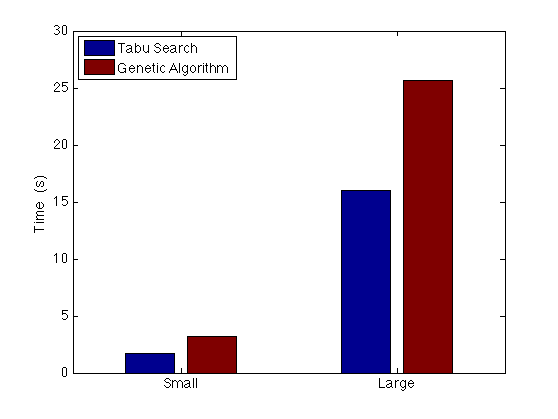
\includegraphics[scale=0.5]{../results/figures/time_bar_graph.png}
  \caption{Running time for the small and large sized problems with both algorithms.}
  \label{time_bar_graph}
\end{figure}

\pagebreak
\subsection{Evaluation score development}
The evaluation score varies during one running of the algorithm as follows: \\\\
\begin{figure}[H]
  \centerline{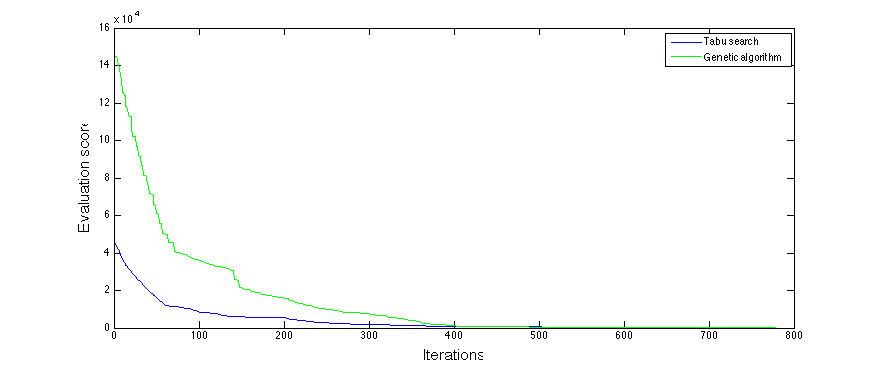
\includegraphics[scale=0.5]{../results/figures/plot_small.png}}
  \caption{Small file.}
  \label{plot_small}
\end{figure}

\begin{figure}[H]
  \centerline{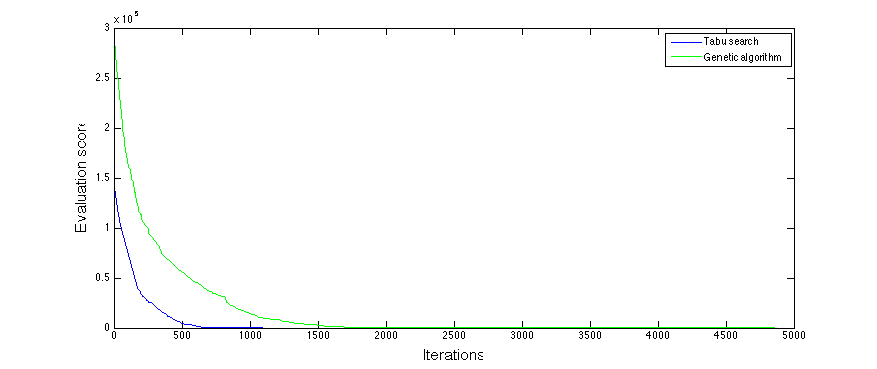
\includegraphics[scale=0.5]{../results/figures/plot_medium.png}}
  \caption{Large file.}
  \label{plot_large}
\end{figure}

\pagebreak
\subsection{Algorithm parameters}
These graphs portray how the running time was influenced by varying the various parameters to the algorithms. More precisely, it shows how long time it took, on an average over 10 runs, to solve the small constraints file when the parameters are varied. \\\\
\begin{figure}[H]
  \begin{center}
    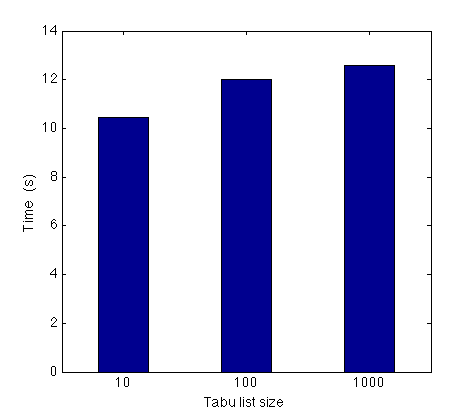
\includegraphics[scale=0.5]{../results/figures/tabu_list_size.png}
  \end{center}
  \caption{The running time of the tabu search for the small file varying the tabu list size.}
  \label{tabu_list_size}
\end{figure}

\begin{figure}[H]
  \begin{center}
    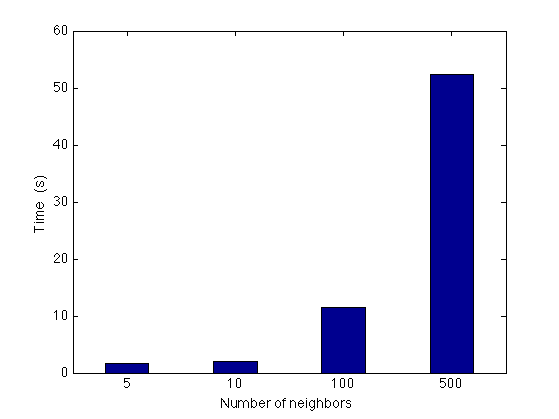
\includegraphics[scale=0.5]{../results/figures/tabu_neighbor.png}
  \end{center}
  \caption{The running time of the tabu search for the small file varying the number of neigbors.}
  \label{tabu_neighbor}
\end{figure}

\begin{figure}[H]
  \begin{center}
    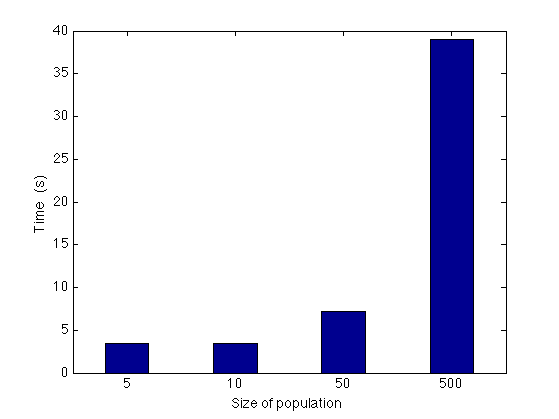
\includegraphics[scale=0.5]{../results/figures/genetic_population.png}
  \end{center}
  \caption{The running time of the genetic algorithm for the small file varying the size of the population.}
  \label{genetic_pop}
\end{figure}

\begin{figure}[H]
  \begin{center}
    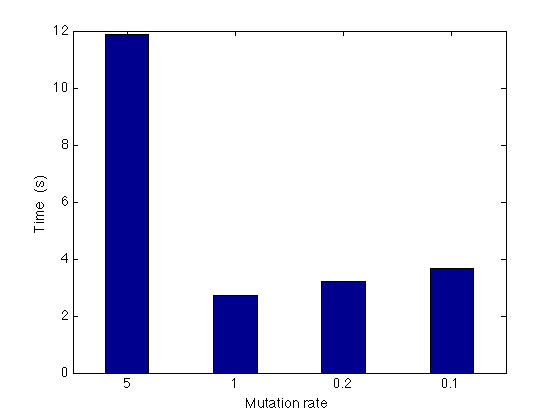
\includegraphics[scale=0.5]{../results/figures/genetic_mutation.png}
  \end{center}
  \caption{The running time of the genetic algorithm for the small file varying the rate of mutation.}
  \label{genetic_pop}
\end{figure}

\begin{figure}[H]
  \begin{center}
    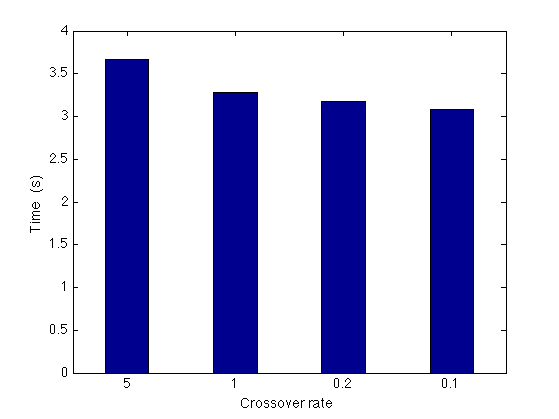
\includegraphics[scale=0.5]{../results/figures/genetic_crossover.png}
  \end{center}
  \caption{The running time of the genetic algorithm for the small file varying the crossover rate.}
  \label{genetic_pop}
\end{figure}

\pagebreak
\section{Discussion}
For the small input size, Tabu Search is significantly faster than our Genetic Algorithm, at about 53\% of the running time. As the size increases, this ratio changes slightly to 62\% of the running time. For the input we have, Tabu Search performs better, however the algorithms does not differ significantly in how well they scale to increasingly large input sizes. Looking at how the evaluation score develops during the running of the algorithm, we can see a clear pattern. The Genetic Algorithm has a worse solution at all times during the run, but when there are only very few broken constraints left, the algorithm is having a lot of trouble satisfying these constraints. This should mean that if we relax the constraints slightly, the genetic algorithm will perform much better. Also notable is a distinct ``corner'' in the Tabu Search graph. It starts out improving very quickly, and then at one point immediately slows down significantly. The Genetic Algorithm has more of a smooth curve where the improvement decreases gradually.
 \\\\
The amount of neighbors generated and visited each iteration in Tabu Search makes the running time vary greatly. When fewer neighbors are evaluated at a time, the Tabu Search runs for more iterations and changes the current optimal solution more often, while less time is spent finding a good neighbor to iterate to. This seems to be more efficient for the input data used in this project.
The Tabu List size, on the contrary, has relatively little impact on the running time. It decreases slightly with larger list sizes. It is possible having a longer Tabu List is simply not worth it due to the larger overhead of dealing with the larger list. \\\\
Varying the population size of the genetic algorithms has a major impact on the time it takes to find an optimal solution. When increasing the size of the population the number of potential solutions managed by the algorithm grows and with that the diversity of the solutions. This could potentially lead to finding better solutions in fewer iterations. However, it appears that the increased time it takes for the algorithm to handle all these solutions outweigh the advantage of a greater diversity among the solutions. \\\\
A higher mutation rate result in more genes being mutated. Although this allows the algorithm to move faster towards a better solution the performance of the algorithm is reduced as extra work has to be put into carrying out the increased number of mutations. Performing too few mutations appears to lower performance as well but not as radically. \\\\
The crossover rate does not have a great impact on the performance of the algorithm. The same principle as in the case of both population size and mutation rate applies here. A higher rate increases solution improvment per iteration but also the time to perform an iteration. It seems as though lowering the crossover rate has a slight performance advantage.\\\\
It should be noted that the implementation of the algorithms certainly has an impact on their running time, as can be seen with the wild variations of running time when some of the algorithm parameters are changed. However, effort has been made to stay close to the most common implementations of the algorithms as described in literature.

\pagebreak
\section{Conclusion}
Tabu Search performs better for all assessed inputs of various sizes. However, the difference is not huge, and the specific implementation and code of the algorithms certainly affect how well they perform, so a general conclusion about the algorithms is hard to draw from this. There is no major difference in how well the different algorithms scale to larger input sizes, and since the specific coding of the algorithms should only affect the running time by some constant, this is a conclusion that can be drawn with greater certainty.

\pagebreak

\bibliographystyle{plain}
\bibliography{sources}
\end{document}